\chapter{Frapi v2: back-end design guidelines}
\label{chap4}

Read-only endpoints built with Frapi and the FracTree ORM are not difficult to maintain. One JSON per resource exposed by the API is sufficient. The scenario changes when dealing with write operations due to new factors of data validation, communication with external systems, business rules checks and modelling of the problem domain.
Frapi class-based custom routes were created as a temporary solution for write operations and were not ideal.

The \texttt{buildEndpoints()} method of endpoint classes is completely flexible, allowing the API developer to design the back end as wanted. This feature became an issue. Frapi applications with similar use cases and the same technology stack were being developed ad-hoc, with diverse standards and code organisation. It was harder for developers from different projects to help teammates due to different setups and ways to solve the same problems.

Used to the ``FENCE way'' of writing programs, the Glance Team started to repeat the same mistakes made on the old framework systems. The learning curve was still something to be aware of. There was a high coupling between new components, a lack of tests and common infrastructure problems were being solved by the team instead of relying on third-party solutions. To avoid migrating the applications to another solution and keeping the same problems, a task force was created to study how the back end was designed in the software industry and propose a series of guidelines to be followed by Frapi systems. The proposed structure should, thus, be strict in the way that multiple applications use the same patterns and are flexible enough to be extended according to the system's needs.

Therefore, Frapi v2 is essentially a shift in how REST APIs are developed using the FENCE module by adding the \textit{controller} endpoint type described in \autoref{sec:controller-endpoints}. The shared structure inspirations, design guidelines and how to apply them will be discussed in depth in the remaining sections.

\section{Controller endpoints}
\label{sec:controller-endpoints}

Controller endpoints are a new way of defining REST API routes on Frapi with the goal of replacing \textit{class endpoints} (\autoref{sec:custom-endpoints}) and solving some of its issues. The previous alternative used direct access to the Slim micro-framework for routing inside the \texttt{buildEndpoints()} function. It created a discrepancy of where routes were registered, \textit{FacTree endpoints} were defined on JSON files while \textit{class endpoints} were defined on PHP classes, usually in different directories, decreasing general maintainability and difficulting for new developers to read the API source code. The direct access to Slim bypassed the abstraction created by Frapi, making future replacements and updates of the framework more difficult and thus affecting the system's extensibility and adding the risk of accumulating technical debt.

\subsection{Route definitions}

To keep consistency with \textit{FacTree endpoints}, the endpoint path and method are configured in JSON files. \nameref{code:controller-endpoint-json} illustrates the configuration of controller endpoints for the Service Work task resource. By defining the \texttt{controller} type and specifying the class, Frapi will instantiate it and call the configured methods according to the received request. Routes are defined under the texttt{paths} parameter, where keys are the URI paths of the endpoints, and the values contain another set of keys corresponding to the HTTP method. The \texttt{method} configuration defines the method of the controller class that will be called when the request is received.

\begin{listing}[htbp]
\begin{minted}{json}
{
    "type": "controller",
    "class": "\\Alice\\ServiceWork\\TaskController",
    "paths": {
        "/tasks": {
            "GET": { "method": "findAllTasks" },
            "POST": { "method": "registerTask" }
        },
        "/tasks/:id": {
	        "GET": { "method": "findTask" },
            "PUT": { "method": "updateTask" },
            "DELETE": { "method": "removeTask" }
        }
    }
}
\end{minted}
\caption{Route definitions of controller-based endpoints.}
\label{code:controller-endpoint-json}
\end{listing}

Following the example, if a client sends a \texttt{GET /tasks} request, Frapi will instantiate a \texttt{Alice\textbackslash ServiceWork\textbackslash TaskController} object and call the \texttt{findAllTasks} method. Observe how multiple routes are registered in an organised and readable manner, helping the developer easily view the available endpoints and which method is executed when they are requested.

The controller class is shown on \nameref{code:controller-endpoint-php}. The controller methods should be public and have an \texttt{Api} object as the first argument, which could be used to get the request and the response objects. The response must be returned at the end of the method to be sent to the client.

\begin{listing}[htbp]
\begin{minted}{php}
<?php

namespace Alice\ServiceWork;

use Fence\Frapi\Api;
use Fence\Frapi\Response;

class TaskController
{
	public function findAllTasks(Api $api): Response
	{
		$request = $api->getRequest();
		// Find task...
		
		$response = $api->getResponse();
		// Write response...

		return $response;
	}

	public function removeTask(Api $api, $id): Response
	{
		// Remove task by ID...
	}

	// Other methods...
}
\end{minted}
\caption{Controller class that handles Service Work task-related requests.}
\label{code:controller-endpoint-php}
\end{listing}

The \nameref{code:controller-endpoint-json} and \nameref{code:controller-endpoint-php} also exemplify how parameters can be used on the URI. In the case of deleting the task with ID 197, it is a common practice in REST APIs to send a request similar to \texttt{DELETE /tasks/197}. Frapi supports this scenario by following the Slim v2 convention \cite{slim-v2-routing-params} with the \texttt{:id} parameter on the endpoint path, which will be used when calling the controller method \texttt{removeTask}.

\subsection{Authorisation}

Controller endpoints also support access control. To protect a route, a permission schema should be added under the \texttt{authorization} key. The authorisation mechanism is identical to the one used by the first version of Frapi on the FacTree endpoints (\autoref{sec:frapi-v1-authorisation}).

\begin{listing}[htbp]
\begin{minted}{json}
{
    "type": "controller",
    "class": "\\Alice\\ServiceWork\\TaskController",
    "paths": {
        "/tasks": {
            "POST": {
	            "method": "registerTask",
	            "authorization": [
                    { "roles": ["admin"] }
                ]
	        }
        },
    }
}
\end{minted}
\caption{Authorisation configuration for controller-based endpoint.}
\label{code:controller-endpoint-auth-json}
\end{listing}

\subsection{Request validation}

To address a shared need between applications to guarantee a correctly formatted HTTP request body, the feature of schema-based validation was introduced to Frapi. The solution consists of checking the requests body JSON against a schema with rules of expected keys, values types and formats, and optional fields defined in the already established JSON Schema standard \cite{json-schema-spec}.

Following the specification, schemas are written in JSON format. Since they usually contain multiple lines of rules and definitions, the design decision was to create a file for each schema. Each is referenced on the controller endpoint file under the \texttt{schema} key as exemplified on \autoref{code:controller-endpoint-schema-json}.

\begin{listing}[htbp]
\begin{minted}{json}
{
	"type": "controller",
    "class": "\\Alice\\ServiceWork\\TaskController",
    "paths": {
		"POST": {
                "method": "registerTask",
                "schema": "resources/schemas/task-register.json"
            }
        }
    }
}
\end{minted}
\caption{Request validation configuration for controller-based endpoint.}
\label{code:controller-endpoint-schema-json}
\end{listing}

\subsection{Dependency injection}
\label{sec:dependency-injection}

Following the example on \autoref{code:controller-endpoint-schema-json}, Frapi internally instantiates the \texttt{TaskController} class and calls the \texttt{registerTask} method as simplified on \autoref{code:controller-call}. The controller instantiation is trivial when it does not have any dependencies.

\begin{listing}[htbp]
\begin{minted}[startinline]{php}
$controller = new \Alice\ServiceWork\TaskController();
$controller->registerTask($api);
\end{minted}
\caption{Controller class instantiation.}
\label{code:controller-call}
\end{listing}

Take \autoref{code:controller-with-dependencies} as an example, which uses the dependency injection (DI) \cite{php-the-right-way-di} pattern, which removes hard-coded dependencies, making it possible to replace them as desired. The controller has two dependencies (database connection and email service) at the constructor level which Frapi would need to resolve somehow similar to \autoref{code:controller-with-dependencies-call}. Without any hints, it is not possible for Frapi to instantiate the dependencies, and also their own dependency tree, to call the controllers.

\begin{listing}[htbp]
\begin{minted}[startinline]{php}
class TaskController
{
	public function __constructor(
		DatabaseConnection $connection,
		EmailService $emailService
	) {
	}

	public function registerTask(Api $api): Response
	{
		// Use database connection and email service
		// to register a task...
	}
}
\end{minted}
\caption{Controller class with dependencies.}
\label{code:controller-with-dependencies}
\end{listing}

\begin{listing}[htbp]
\begin{minted}[startinline]{php}
$connection = new DatabaseConnection($dsn, $user, $password);
$emailService = new EmailService($credentials);
$controller = new TaskController($connection, $emailService);
\end{minted}
\caption{Manual instantiation of the controller class.}
\label{code:controller-with-dependencies-call}
\end{listing}

To address the need for automatically injecting dependencies, the second version of Frapi introduced support for DI containers. The container is a tool to make the injection more practical by letting the application define how classes and interfaces should be created and by instantiating and injecting them. It was decided not to rely on any specific third-party tool but instead use PSR-11 \cite{psr-11} containers. PHP Standard Recommendations (PSRs) are a set of interfaces created by the Framework Interoperability Group (FIG) \cite{fig-website} to standardise the commonalities between established PHP projects. All the major PHP DI container libraries follow the container interface from PSR-11, allowing Frapi applications to choose between a wide range of tools according to their needs.

Frapi uses the DI container provided by the application to create the controllers. The container is sent to Frapi via the texttt{setContainer()} method as shown on \autoref{code:set-container-example}. PHP-DI \cite{php-di} is used in the example, but any other PSR-11 container could be used.

\begin{listing}[htbp]
\begin{minted}[startinline]{php}
$containerBuilder = \DI\ContainerBuilder();
$containerBuilder->addDefinitions([
	DatabaseConnection::class => function () {
		return new DatabaseConnection(
			getenv(DB_CONNECTION_STRING),
			getenv(DB_USERNAME),
			getenv(DB_PASSWORD)
		);
	},
	EmailService::class => function () {
		return new EmailService(getenv("EMAIL_CREDENTIALS"));
	},
]);
$container = $containerBuilder->build();

$api = new Api("configuration.json");
$api->setContainer($container);

$api->run();
\end{minted}
\caption{Dependency injection definitions and usage example of the \texttt{setContainer} method.}
\label{code:set-container-example}
\end{listing}

\section{Framework independence}

The remaining sections will no longer describe Frapi features and internal behaviour but instead focus on creating guidelines to design better and set standards for back ends across the Glance Team due to common problems and use cases. The individualities of each project were also kept in mind, resulting in the need for flexible guidelines.

At this point, the bottleneck of development speed and maintenance created by FENCE was well-known around the team. The first decision of the guidelines was to not rely heavily on a framework. Frameworks help create simple CRUD applications rapidly and have large communities, providing a significant amount of support and documentation. However, their generalist nature conflicts with the need to create systems with complex rules. What at first was a tool which enabled fast bootstrapping became an obstacle for developers to evolve the application around the framework.

Notice that frameworks were not banned. Applications could use them but were strongly advised to avoid using external libraries at the core of their projects. Regarding FENCE, the team decided to avoid almost everything from the in-house and use external libraries for common problems. Since Frapi was packed inside FENCE, its usage was allowed. The Logger was inspired by PSR-3 \cite{psr-3} and could be replaced without much work. It was discouraged the usage of other classes and features from FENCE, such as \texttt{Configuration}, FacTree models and \texttt{Utils}.

\section{Domain-Driven Design}
\label{sec:ddd}

Frapi applications started as an interface to external systems to consume Glance data. With the decision to develop applications with decoupled front-end and back-end layers, REST APIs would need to handle all read-and-write use cases. It was already known that the new projects would not have to deal with simple CRUD operations but would need to implement all the complex business rules and processes unique to the collaboration of each experiment. Based on the problems of creating purely in-house solutions and developing ad-hoc, the team researched to find existing patterns which could be used as a base for building complex software systems.

Domain-Driven Design (DDD) was the main inspiration for the back-end guidelines. It is a set of principles initially defined in the book \textit{Domain-Driven Design: Tackling Complexity in the Heart of Software} written by Eric Evans in 2003 \cite{ddd-blue-book}. The author proposes developing software solutions centred on the domain model with a great understanding of the rules and flows of the business. It fits the needs of systems similar to the ones built by Glance Team, which provide solutions to complex domains with messy logic to be organised \cite{ddd-martin-folwer}. Since the first publication, the principles gained adoption, were put into practice and evolved. The methodology became particularly popular among microservices, helping to split a system into smaller services by identifying the responsibilities and relations of each.

The DDD methodology is divided into two phases: Strategic and Tactical Design. The former involves a deep understanding of the business and defining responsibilities and boundaries among modules. It should answer \textit{what} and \textit{why} is the software solution being built. The latter focuses on \textit{how} to translate the knowledge extracted from the first phase into code by defining building blocks. The blocks, such as entities, value objects, aggregates, services, repositories, and events, will be explained briefly on \autoref{sec:building-blocks}. For an in-depth explanation of each pattern, it recommended the read of Evans' original text \cite{ddd-blue-book} and Vaughn Vernon's \textit{Implementing Domain-Driven Design} book \cite{ddd-red-book}.

The Strategic Design suggests breaking the domain, which may be broad and abstract, into smaller pieces called \textbf{subdomains} \cite{petter-holmstrom-part1}. Subdomains can be classified as \textbf{core}, \textbf{supporting}, and \textbf{generic}. Core subdomains are the most important, special and unique parts of the domain. They are the reason for the existence of the system. Generic subdomains are the pieces that are unrelated to the organisation and can be replaced by third-party solutions but are still needed for the operation of the overall solution. Supporting subdomains are the ones which are not part of the main goal of the solution but are also not generic enough since they require specific context about the organisation. For example, on the Service Work system, the ALICE task management domain was split into seven subdomains as illustrated on \autoref{fig:sw-subdomains-diagram}. The \textit{Task} subdomain encompasses the management of tasks, including planning and assignments. It is categorised as core because it is vital to Service Work. \textit{Institutions} is an example of a supporting subdomain. It includes the modelling of institutes, clusters and service clusters of the ALICE collaboration, containing specific knowledge of the domain but not being its core. Finally, generic subdomains are exemplified by \textit{Identity and Access} and \textit{Notification}. Both parts do not contain any logic unique to CERN, ALICE or Service Work and could be replaced by off-the-shelf solutions but are essential for the overall workflow of the system.

\begin{figure}[htbp]
  \centering
  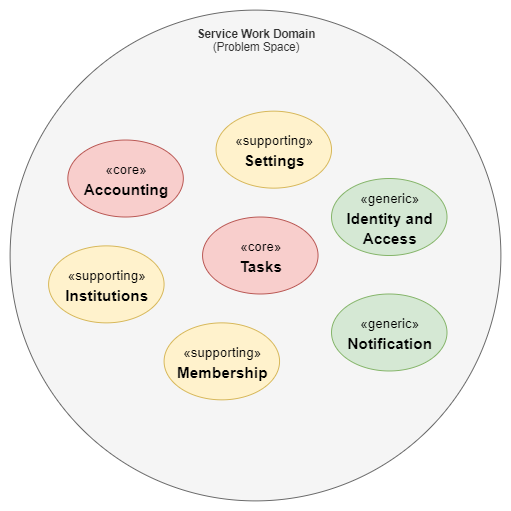
\includegraphics[scale=0.6]{Imagens/chap04/sw-subdomains-diagram.png}
  \caption{Subdomains of the Service Work problem space.}
  \label{fig:sw-subdomains-diagram}
\end{figure}

Evans \cite{ddd-blue-book} also advocates the use of \textbf{ubiquitous language}. It is a language shared by developers and domain experts to describe the problem and the solution. Most of this language comprises the terminology used by the business or in the ALICE experiment following the Service Work example. The idea behind this concept is also to use this language to model the solution and write the software, thus reducing the communication barrier of translating technical code to domain processes.

Moving to the solution space, Domain-Driven Design also defines the concept of \textbf{bounded contexts}. Like subdomains, bounded contexts are parts of the domain, the difference being that the latter corresponds to a division on the solution space instead of the problem space. Usually, there is a one-to-one mapping between subdomains and bounded contexts, but this is not a rule. It is possible to have a single subdomain with multiple bounded contexts and vice-versa.

Understanding, discovering, decomposing and organising subdomains is not trivial and requires a deep knowledge of the entire problem space. It is crucial to first understand the problem before trying to solve it, turning communication with domain experts of great importance. Multiple techniques exist to help developers and experts visually and collaboratively map the domain \cite{ddd-modelling-process}. The exploration of the Service Work domain was done using the Event Storming \cite{event-storming-website} \cite{introducing-event-storming} approach. It consists of a brainstorm of domain \textbf{events}. An event is something meaningful that happened on the domain and is represented by orange sticky notes (see \autoref{fig:event-storming-sw-zoom-in}). Later, the \textbf{commands} that triggered the events blue notes are added before the events and with yellow notes representing the \textbf{actor} who performed the action. Finally, the sticky notes are rearranged and linked through arrows indicating that a command is triggered due to an event. If there is a condition to continue the workflow, it is represented as a purple after the event note.

\begin{figure}[htbp]
  \centering
  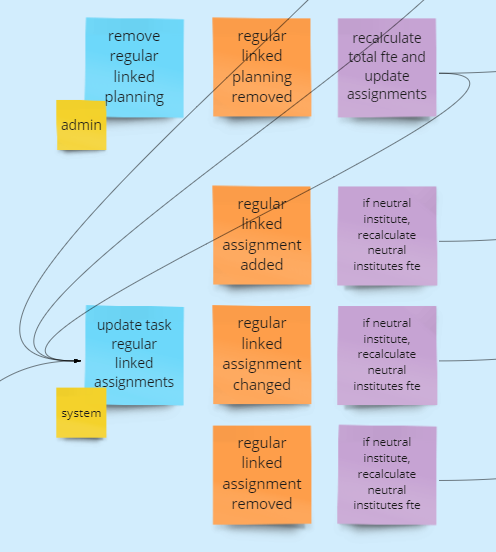
\includegraphics[scale=0.7]{Imagens/chap04/event-storming-sw-zoom-in.png}
  \caption{Details of the event storming board from Service Work.}
  \label{fig:event-storming-sw-zoom-in}
\end{figure}

Using Event Storming at Service Work facilitated the strategic design of the system. The approach helped discover events, use cases, user personas, and separation of subdomains and made it easier to visualise the various complex flows of the system. \autoref{fig:event-storming-sw-zoom-out} illustrates part of the result of event storming. Note how events were organised, permitting to draw the boundaries of the two core subdomains.

\begin{figure}[htbp]
  \centering
  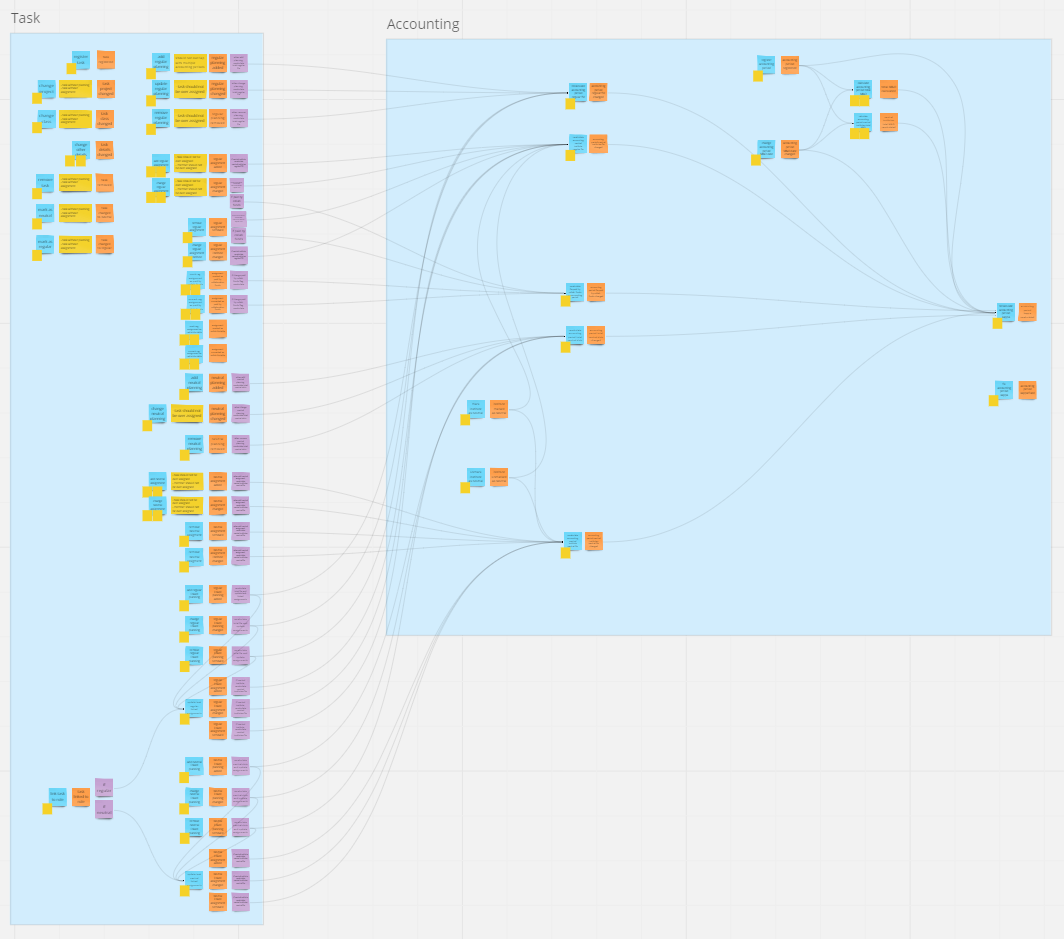
\includegraphics[scale=0.5]{Imagens/chap04/event-storming-sw-zoom-out.png}
  \caption{Part of the result of event storming at Service Work.}
  \label{fig:event-storming-sw-zoom-out}
\end{figure}

\section{Architecture}

Software architecture can be defined as the division of the system into smaller units, the relation between those components, their characteristics and how they are arranged \cite{sven-woltmann-hexagonal-architecture}. When the Glance Team started to create decoupled applications, the developers agreed that the chosen architecture must facilitate system changes. The addition or replacement of business rules, modernisation of technologies and infrastructure upgrades should be done with little and predictable effort, with explicit consequences and no hidden side effects. This characteristic should be kept up in the software during its lifetime. In other words, the Glance applications would need to be operational and maintainable for at least 20 years, during which the LHC experiments are planned to run \cite{lhc-end-of-life}.

\subsection{Layered Architecture}
\label{sec:layered-architecture}

At the beginning of the development of the first Frapi-based REST APIs, the Glance Team adopted the \textit{Layered Architecture}. Also known as \textit{n-tiered}, this architectural style organises the system components in horizontal layers with distinct roles. It mostly adopted with the \textbf{presentation}, \textbf{business}, \textbf{persistence} and \textbf{database} layers, but there is no limitation in the number and type of layers \cite{richards-architecture}. \autoref{fig:layered-architecture-on-frapi} exemplifies how Layered Architecture was used where the blue containers represent the deployable units, layers are represented in orange with their components in green. The presentation layer was responsible for handling the communication with the API consumers. \textbf{Controller} classes would parse HTTP requests, coordinate the call of business logic and later format responses. The business layer executes a \textbf{Service} with specific domain rules and flows without validating the input from the users since this is the responsibility of the previous layer. Similarly, it does not have to know how to retrieve the data and reconstruct an \textbf{Entity} since it is the responsibility of the \textbf{Repository} on the persistence layer, which communicates with the datastore on the database layer. Each layer could be tested in isolation by mocking components and other layers, facilitating the development of automated tests.

\begin{figure}[htbp]
  \centering
  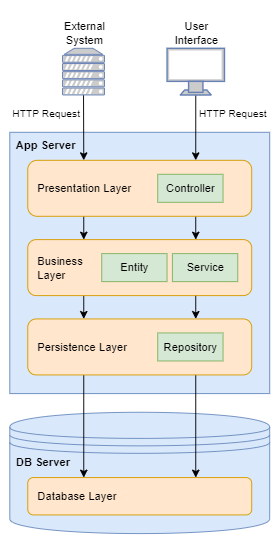
\includegraphics[scale=0.55]{Imagens/chap04/layered-architecture-on-frapi.png}
  \caption{Layered architecture diagram.}
  \label{fig:layered-architecture-on-frapi}
\end{figure}

Due to its simplicity, the Layered Architecture has low development cost and is well suited for small and simple applications. However, as the Glance APIs increased their inherent complexity, maintainability was affected. By being technically partitioned, components were grouped by their technical function instead of their business role \cite{richards-architecture}. It became challenging to reason about the complex domain constraints and processes when everything was partitioned on the same layer. The style also induces developers to a data-driven design, with the software being built around how the database is structured and the relation between tables. By focusing on how data is persisted instead of modelling the business and its behaviour, the approach moved away from the desired domain-driven design.

\subsection{Hexagonal Architecture}
\label{sec:ports-and-adapters}

With the downsides of Layered Architecture, the team went back to research a new architectural style that would better fit with domain-driven design due to the business complexity of the systems. The chosen solution was the \textit{Ports and Adapters Architecture}, also known as \textit{Hexagonal Architecture}, proposed by Alistair Cockburn in 2005 \cite{alistair-cockburn-hexagonal-architecture}. It defends that the business logic should be developed in isolation, allowing the system to be equally used by users, external services and test runners. The use cases and business logic are encapsulated at the core of the architecture called \textbf{application} as illustrated on \autoref{fig:ports-and-adapters-diagram}. On this layer, \textbf{ports} serve as an interface to external components such as users, REST API clients, databases, filesystem and third-party APIs. The connection with the outside world is made on the outer layer of the hexagon via \textbf{adapters}, which implement the port interfaces. \textit{Driving} ports and adapters control the application are represented on the left side of the diagram, while the \textit{driven} components are placed on the right side \cite{sven-woltmann-hexagonal-architecture}. The style defined by Cockburn is almost identical to Robert Martin's \textit{Clean Architecture} \cite{robert-martin-clean-architecture-book} and Jeffrey Palermo's \textit{Onion Architecture} \cite{onion-architecture-article}.

\begin{figure}[htbp]
  \centering
  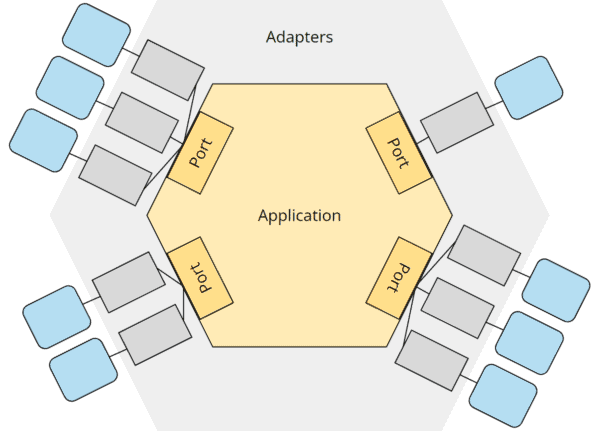
\includegraphics[scale=0.5]{Imagens/chap04/ports-and-adapters-diagram.png}
  \caption{Ports and adapters components on the hexagonal architecture \cite{sven-woltmann-hexagonal-architecture}.}
  \label{fig:ports-and-adapters-diagram}
\end{figure}

Note how the control of the system on this architecture flows from left to right: it starts on the driving components, going to the corresponding adapters and ports, calling the business logic which then uses the driven components by using their corresponding ports implemented by adapters. The source code dependency, however, is different, as shown on the left diagram of \autoref{fig:hexagonal-architecture-vs-layered-architecture-diagrams}. All the components of this architecture depend on their current or inner layers. The business is the central part, everything depends on it, but the domain code has no dependencies, turning it technically simple and allowing it to focus on modelling the complex business. This dependency characteristic facilitates the domain-driven design approach in contrast with the Layered Architecture in which the components' dependencies points to the database layer, as illustrated on the right diagram of \autoref{fig:hexagonal-architecture-vs-layered-architecture-diagrams}.

\begin{figure}[htbp]
  \centering
  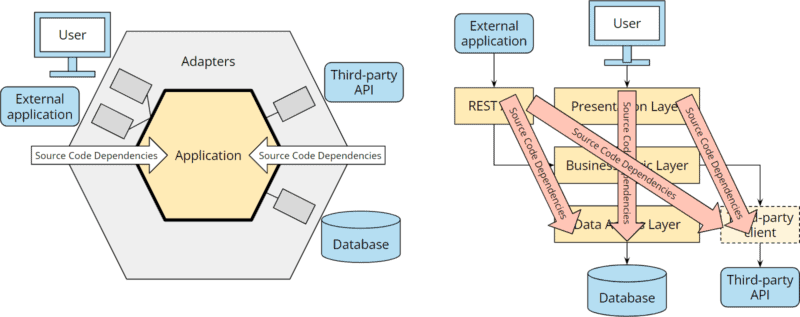
\includegraphics[scale=0.5]{Imagens/chap04/hexagonal-architecture-vs-layered-architecture-diagrams.png}
  \caption{Comparison between \textit{Ports and Adapters} and \textit{Layered} architectures \cite{sven-woltmann-hexagonal-architecture}.}
  \label{fig:hexagonal-architecture-vs-layered-architecture-diagrams}
\end{figure}

The Ports and Adapters Architecture allows easy modifying or even replacing adapters. This is an advantage since it brings the possibility of changing infrastructure components such as databases, upgrading dependencies, and also performing tests by using mock adapters without much effort. Another benefit of Hexagonal Architecture is that the team can start developing and modelling the domain code without having to know about what infrastructure components will be used, such as frameworks and database types, and delaying this decision to a later stage with a mature project and a clearer vision of the system needs \cite{sven-woltmann-hexagonal-architecture}.

\subsection{Modular Monolith}
\label{sec:modular-monolith}

To avoid the issues of a technically partitioned exposed on \autoref{sec:layered-architecture}, the Glance Team decided to divide the system in bounded contexts (\autoref{sec:ddd}), reflecting the subdomains of the problem space. Contexts are independent modules and follow the Ports and Adapters architectural style. \autoref{fig:multiple-bounded-contexts} illustrates this topology with three bounded contexts, each represented by a hexagon. Each module can consume data from databases, external APIs and even other internal models. As a guideline, modules should not directly depend on other bounded context components but instead make use of ports and adapters. 

\begin{figure}[htbp]
  \centering
  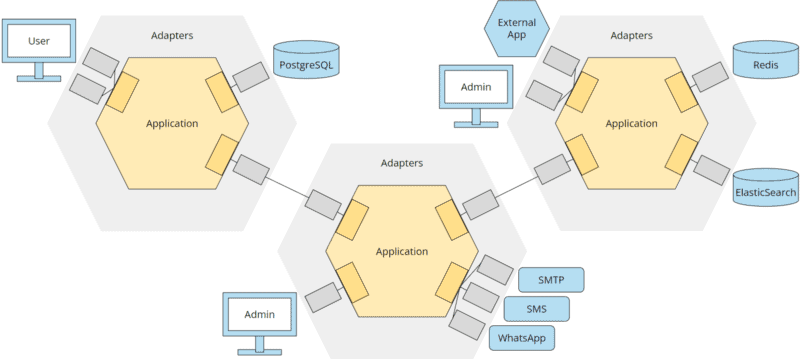
\includegraphics[scale=0.5]{Imagens/chap04/multiple-bounded-contexts.png}
  \caption{Multiple bounded contexts on the hexagonal architecture \cite{sven-woltmann-hexagonal-architecture}.}
  \label{fig:multiple-bounded-contexts}
\end{figure}

Even though the Hexagonal Architecture is well suited for distributed microservices, the Glance Team agreed to use at first a \textbf{monolithic topology}. The nonfunctional characteristics of distributed computing, such as performance, scalability and availability, were not typical requirements for the projects being developed. Creating multiple deployable units would bring unnecessary technical complexity and other groups of issues, such as the fallacies of distributed computing, described by Peter Deutsch and James Gosling in 1994 and 1997 \cite{fallacies-of-distributed-computing} \cite{richards-architecture}. The benefits of microservices for big teams were also not applicable since the development teams for each Glance system are usually from one to three members.

Unlike a classic monolith such as FENCE systems, the proposed topology is a \textbf{modular monolith}. The system comprises modules (bounded contexts) forming a single deployable package. Contexts do communicate with each other internally on the same thread and programming language (PHP) by using ports and adapters as if they were distributed to avoid high coupling. It is also possible to perform internal communication via REST API requests, but this is unnecessary, resulting in a loss of performance without any gain.

The same reasons for not using microservices apply to databases. A common solution may use one persistence mechanism per module to isolate data. For simple deployments, easy maintenance and considering the low number of developers, the Glance team decided to use at first one database per system. It could be split into several databases if needed in the future. To preserve data isolation, the database may be divided logically by bounded context, for example, by adding a module prefix to each table name and discouraging the usage of tables from outside the module.

\autoref{fig:service-work-topology} illustrates a simplified version of the Service Work system topology. It is composed of four deployable units in blue: \textit{front end}, \textit{back end}, \textit{database} and \textit{job scheduler}. The back end is an example of a modular monolith composed of seven bounded contexts reflecting the subdomains of the business (\autoref{fig:sw-subdomains-diagram} on \autoref{sec:ddd}). Modules communicate internally with each other and also use external resources such as the database, third-party APIs (CERN Authorization Service) and legacy systems. In this case, the Membership bounded context works as an anticorruption layer \cite{ddd-blue-book} to access a legacy system. Observe how the database is logically divided into parts used only by their corresponding modules. Clients like the front and external systems can call the back end via HTTP, while the job scheduler uses a command line interface.

\begin{figure}[htbp]
  \centering
  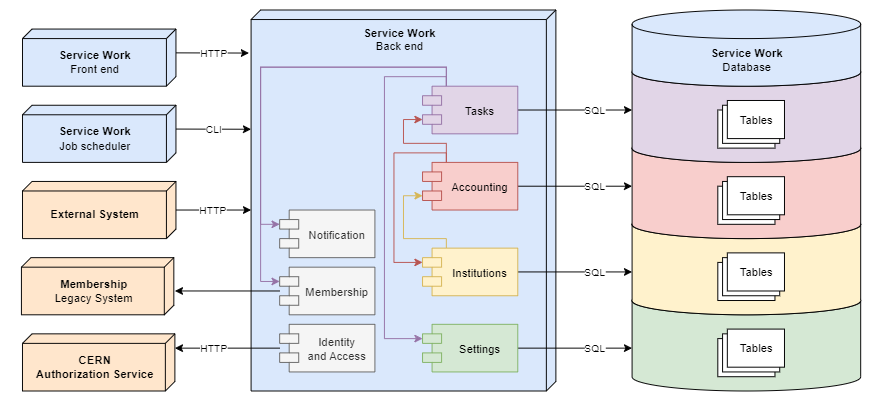
\includegraphics[scale=0.48]{Imagens/chap04/service-work-topology.png}
  \caption{The modular monolith topology of the Service Work system.}
  \label{fig:service-work-topology}
\end{figure}

\section{Building blocks}
\label{sec:building-blocks}

The current section describes recommended building blocks for implementing Glance REST APIs. As the entire guideline, this is not a definitive list with immutable rules. Exceptions can exist, and better ways of developing complex applications may be proposed. The blocks are patterns and best practices from object-oriented programming and may be found in the literature with different names depending on the reference. On the DDD scope, they are divided into three layers: \textbf{domain}, \textbf{application} and \textbf{infrastructure}. 

\subsection{Domain}

Domain objects are used to model the business and express its logic. This layer consists of simple and isolated classes without dependency on infrastructure, user interface and application code. Without other responsibilities, domain objects can focus purely on reflecting all the nuances of the problem space with rich detail on all essential constraints, behaviours and events.

\subsubsection{Value Object}
\label{sec:value-object}

Value objects \cite{ddd-blue-book} \cite{ddd-reference} are used to represent measurable, quantifiable values or to simply describe concepts in an easier way to test, use and maintain \cite{ddd-red-book}. These objects model the domain and care about their values instead of their identity. Take, for example, a 2-dimensional coordinate represented by points X and Y. The point (1,4) equals any other point with $X = 1$ and $Y = 4$. In this case, it makes sense to model coordinates as a value object \cite{fowler-value-objects}. On the other hand, two different individuals named ``Eric ''may not be the same person. If a person changes their name, it remains the same person. Thus their identity matters, and value objects may not be the best choice to model a person.

On Service Work, FTE (Full-Time Equivalent) represents the work planned or assigned to a task. 1 FTE is the maximum amount of work of a collaboration member. 1 FTE during one day equals 8 working hours, but 1 FTE during a week equals 40 work hours. \autoref{code:fte-example} illustrates how the application uses value objects to model a domain concept. Instead of representing FTEs as primitive float values, a class was created. Note how the domain constraint of FTEs being always positive is enforced at the constructor level. This design eliminates the need for validating this rule anywhere else in the system.

\begin{listing}[htbp]
\begin{minted}[startinline]{php}
class Fte
{
	public function __construct(
		public readonly float $value
	) {
		if ($value <= 0) {
			throw new \Exception("FTE must be positive.");
		}		
	}

	public function equals(Fte $otherFte): bool
	{
		return $this->value === $otherFte->value;
	}

	public function add(Fte $fte): Fte
	{
		$sum = $this->value + $fte->value;
		return new self($sum);
	}
}
\end{minted}
\caption{Value object to model the domain concept of FTE.}
\label{code:fte-example}
\end{listing}

Value objects can contain other value objects. Continuing the Service Work narrative, if a task is planned to have 0.5 FTEs during 6 months, a member of the ALICE collaboration should work half-time for six months to complete this task. Other combinations, such as working full-time for three months, are also possible. The \texttt{FtePeriod} class on \autoref{code:fte-period-example} illustrates how the combination of FTEs and a date period can be modelled. It enforces the domain rule that FTE periods should start and end at the corresponding month's start and end dates. It is also immutable. Any change on a value object implies the creation of a new object, preventing side effects. The immutability is exemplified by the methods \texttt{withFte} and \texttt{withPeriod}.

\begin{listing}[htbp]
\begin{minted}[startinline]{php}
class FtePeriod
{
	public function __construct(
		public readonly Period $period,
		public readonly Fte $fte,
	) {
		if (!$period->startsAtFirstDayOfMonth()) { /* ... */ }
		if (!$period->endAtLastDayOfMonth()) { /* ... */ }
	}

	public function withFte(Fte $fte): self
	{
		return new self($this->period, $fte);
	}

	public function withPeriod(Period $period): self { /* ... */ }

	/* ... */
}
\end{minted}
\caption{Value object to model the domain concept of FTE Period.}
\label{code:fte-period-example}
\end{listing}

\subsubsection{Entity}

Entities are objects defined and distinguished by their identity instead of their attributes \cite{ddd-blue-book}. Following the same example from \autoref{sec:value-object}, if a class is created to model members of the ALICE collaboration, we cannot say that two member objects with the name field “Robert” are the same because people are not fully distinguishable by their name. And if a member changes their name, it remains the same person. Even with different attributes, if two entity objects reference the same identity, they should be considered equal. Different from value objects, entities are mutable and preserve state.

Moving away from a data-centric approach, entities are not modelled with the database in mind. The idea is to create rich classes full of behaviour and domain context. Properties and methods are meaningful, with the same terms domain experts use and without technical names. The idea is to avoid an anaemic domain model \cite{ddd-blue-book} \cite{martin-fowler-anemic-domian-model} made majoritarian of getters and setters, mirroring the database table structure. Without the distractions and technicalities of frameworks, complex domain ideas become simple. The easiness of reading and reasoning about the domain allows rapid additions and changes of business rules on the code.

\autoref{code:entity-task-example} illustrates a simplification of the \texttt{Task} entity from the Service Work application. The properties consist of native PHP types (\texttt{\$name}), value objects (\texttt{\$id}) and other entities (\texttt{\$plannings} and \texttt{\$assignments}). Notice that there are no explicit getters and setters usually found on CRUD-like applications. Instead, there are domain-rich methods full of behaviour and context.

\begin{listing}[htbp]
\begin{minted}[startinline]{php}
class Task
{
	private TaskId $id;
	private string $name;
	/** @var Planning[] */
	private array $plannings;
	/** @var Assignment[] */
	private array $assignments;

	public static function register(TaskId $id, string $name): self {
        /* ... */
    }
	public function plan(FtePeriod $ftePeriod): void {
        /* ... */
    }
	public function assign(MemberId $assignee, FtePeriod $ftePeriod): void {
        /* ... */
    }
	public function unassign(AssignmentId $assignmentId): void { /* ... */ }

	public function isPlannedOnPeriod(Period $period): bool { /* ... */ }
	public function assignableFteOnPeriod(Period $period): Fte { /* ... */}
}
\end{minted}
\caption{Entity to model the domain concept of a Service Work Task.}
\label{code:entity-task-example}
\end{listing}

In systems with complex associations between entities, it becomes difficult to guarantee the consistent state of objects. Evans \cite{ddd-blue-book} \cite{ddd-reference} suggests clustering entities into \textbf{aggregates} with well-defined boundaries. The main entity of the cluster is called \textbf{aggregate root}, and it is the only entity that external objects reference. Persistence and other transactions are made on the entire aggregate. Internal entities are invisible to the outside world of the aggregate boundary, thus making the responsibility of the root to manage and enforce the invariants of the aggregate as a whole.

Continuing with the Service Work example, tasks have multiple planning and assignments on which business rules are enforced. For example, the total FTE assigned to a task should not exceed the FTE planned for the same period. To guard all domain constraints, the Task aggregate boundary was designed around the \texttt{Task}, \texttt{Planning} and \texttt{Assignment} entities as illustrated on \autoref{fig:task-aggregate-boundary}. The \texttt{Task} class is the aggregate root, meaning that planning and assignments are created, exposed and managed by the root entity. When a task is saved, everything on the aggregate is persisted. It is not possible, for example, to save an assignment on the database without updating the whole task. This preserves the task's domain constraints. 

\begin{figure}[htbp]
  \centering
  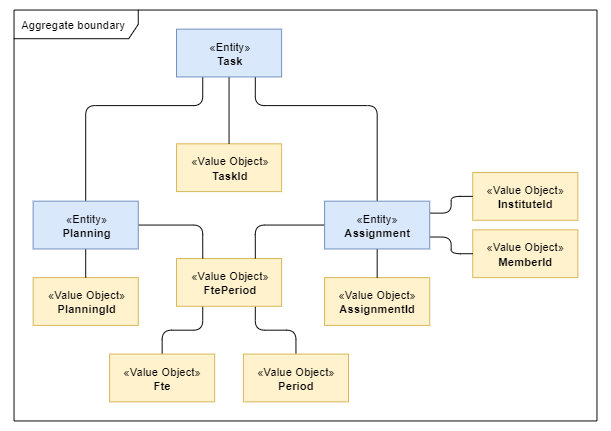
\includegraphics[scale=0.67]{Imagens/chap04/task-aggregate-boundary.png}
  \caption{The modular monolith topology of the Service Work system.}
  \label{fig:task-aggregate-boundary}
\end{figure}

\subsubsection{Domain Event}

Domain events model information about state changes relevant to domain experts. Each event is represented by a domain object \cite{ddd-reference} \cite{ddd-red-book}. This modelling tool allows informing other parts of the application that something happened in the domain via publish-subscribe patterns. Since events represent something that occurred in the past, their objects are immutable and contain only relevant information about the specific activity, such as the identity of the entities involved and the timestamp of when it occurred. The most common use case for events on Glance applications is to send emails when something happens.

When a task is planned on Service Work, the sum of FTE planned for the entire ALICE collaboration should be recalculated and must trigger a notification to the Service Work Coordinator. This event is modelled by the \texttt{TaskPlanned} object exemplified on \autoref{code:task-planned}. Notice how small, simple and immutable the event class is.

\begin{listing}[htbp]
\begin{minted}[startinline]{php}
class TaskPlanned
{
	public readonly DateTimeImmutable $whenOccurred;

	public function __construct(
		public readonly TaskId $taskId,
		public readonly PlanningId $planningId,
		public readonly FtePeriod $ftePeriod
	) {
		$this->whenOccurred = new DateTimeImmutable("now");
	}
}
\end{minted}
\caption{Event to model the domain concept of ``a task was planned''.}
\label{code:task-planned}
\end{listing}

\autoref{code:domain-event-on-entity} illustrates how the command of \texttt{plan} triggers the creation of the event. The method \texttt{registerEvent} keeps all activity with the entity during the request. Events are later released by \texttt{releaseEvents} to be added to an \textbf{Event Publisher}, which will be explained on \autoref{sec:event-subscriber}.

\begin{listing}[htbp]
\begin{minted}[startinline]{php}
class Task
{
    // ...

    public function plan(PlanningId $planningId, FtePeriod $ftePeriod): void
    {
	    // Check if task can be planned with the given FTE during the period...

		$this->planning[] = Planning::register($planningId, $ftePeriod);

		$event = new Event\TaskPlanned($this->id, $planningId, $ftePeriod);
		$this->registerEvent($event);
    }

	public function registerEvent($event): void
	{
		$this->events[] = $event;
	}

	public function releaseEvents(): array
	{
		$events = $this->events;
		$this->events = [];

		return $events;
	}
}
\end{minted}
\caption{Example of the \texttt{Task} entity coordinating the \texttt{TaskPlanned} event.}
\label{code:domain-event-on-entity}
\end{listing}

\subsubsection{Repository}
\label{sec:repository-interface}

Repositories on the domain layer are interfaces that abstract the persistence of aggregates, creating the illusion to consumers that all objects are stored as an in-memory collection \cite{ddd-blue-book}. Each aggregate should have its repository with meaningful methods respecting the ubiquitous domain language. Entities and value objects should not use repositories since querying and persisting are not part of their responsibility. Repositories are usually used by application and domain services. The \texttt{TaskRepository} from \autoref{code:task-repository} exemplifies the repository interface for the Task aggregate.

\begin{listing}[htbp]
\begin{minted}[startinline]{php}
interface TaskRepository
{
    public function save(Task $task): void;
    public function delete(TaskId $id): void;

    /** @return Task[] */
    public function findAll(): array;
    public function findById(TaskId $id): Task;
	/** @return Task[] */
	public function findByMember(MemberId $memberId): array;
    /** @return Task[] */
	public function findPlannedOnPeroid(Period $period): array;
}
\end{minted}
\caption{Task repository interface.}
\label{code:task-repository}
\end{listing}

The repository interfaces are later implemented on the infrastructure layer, allowing the developers to focus first on modelling the complex domain and decide, with a mature project, the ideal persistence strategy. The domain logic and all the application use cases can be first developed without setting up a database. The usage of interface for repositories results in the increase of the general maintainability of the application. The database technology can be later replaced with another without affecting the domain logic. The development work for the change would occur only on the infrastructure code. Another benefit is allowing in-memory repositories that could be used on initial development and for writing automated tests as exemplified on \autoref{code:task-inmemory-repository}.

\begin{listing}[htbp]
\begin{minted}[startinline]{php}
class InMemoryTaskRepository implements TaskRepository
{
	/** @var Task[] */
	private array $tasks = [];

	public function save(Task $task): void
	{
		$id = $task->id()->toInteger();
		$this->tasks[$id] = $task;
	}

	public function findAll(): array
	{
		return $this->tasks;
	}

	public function findById(TaskId $id): Task
	{
		return $this->tasks[$id->toInteger()];
	}

	// ...
}
\end{minted}
\caption{In-memory implementation of the \texttt{TaskRepository}.}
\label{code:task-inmemory-repository}
\end{listing}

\subsection{Application}

The use cases of the system are placed on the application layer. Use cases are modelled so that they are not dependent on the actor who invoked them so that the same logic can be called via HTTP requests, CLI commands or any other type of user input. Application encapsulates and protects the domain code being an interface to any actor willing to command the system. The application layer depends on itself and the domain layer. It focuses on coordinating the business objects to conceive multiple use cases without depending on the infrastructure code.

\subsubsection{Command}
\label{sec:command}

Commands are simple objects used to model the use case input. It ensures that all the required fields are present and in the correct format. It removes the data validation responsibility from the application logic, leaving it with a focus on coordinating and executing the use case. \autoref{code:assign-task-command} illustrates a command for assigning tasks on the Service Work system. The command class does not contain behaviour and functions as a Data Transfer Object (DTO) to carry input information from the infrastructure to the application layer.

\begin{listing}[htbp]
\begin{minted}[startinline]{php}
class AssignTaskCommand
{
	public function __construct(
    	public readonly TaskId $taskId,
    	public readonly MemberId $memberId,
    	public readonly InstituteId $instituteId,
    	public readonly FtePeriod $period,
	) {
	}
}
\end{minted}
\caption{Class to model the command for assigning a task.}
\label{code:assign-task-command}
\end{listing}

Since the system has multiple entry points, such as the RESTful API and CLI commands, each of them should be responsible for validating the format of the input and creating command objects that will be the arguments of the \textbf{Command Handlers} (\autoref{sec:command-handler}) as shown on \autoref{code:task-controller-assign-command}.

\begin{listing}[htbp]
\begin{minted}[startinline]{php}
class TaskController
{
	public function assignTask(Api $api, int $taskId): Response
	{
		$body = $api->getRequest()->getBody();
		$input = json_decode($body);

		// Validate input...

		$command = new AssignTaskComand(
			TaskId::fromInteger($taskId),
			MemberId::fromInteger($input["member_id"]),
			InstituteId::fromInteger($input["institute_id"]),
			new FtePeriod($start, $end, $fte),
		);

		$this->assignHandler->execute($command);
	}
}
\end{minted}
\caption{Usage of the \textit{Command} object on the controller.}
\label{code:task-controller-assign-command}
\end{listing}

\subsubsection{Command Handler}
\label{sec:command-handler}

The command handler is the class responsible for effectively executing the use case. It receives a command object (\autoref{sec:command}) and coordinates domain objects to do what it proposes. There is one handler per use case, and they may call other command handlers.

\autoref{code:assign-task-handler} illustrates how the \texttt{AssignTaskHandler} uses domain objects such as entities, value objects, events and repositories to assign a member to a task. Since the repository is an interface, it can be replaced by in-memory repositories to prototype use cases and write automated tests executed in milliseconds without communicating with databases. Domain events are released from entities and dispatched via the \texttt{EventDispatcher} to allow subscribed listeners to execute new flows based on what occurred.

\begin{listing}[htbp]
\begin{minted}[startinline]{php}
class AssignTaskHandler
{
	public function __construct(
		private TaskRepository $taskRepository,
		private EventDispatcher $eventDispatcher,
	) {
	}

	public function execute(AssignTaskCommand $command): void
	{
		$task = $this->taskRepository
                     ->findById($command->taskId);

		// Used to validate if member is not overassigned
		$memberTasks = $this->taskRepoisitory
                            ->tasksByMember($command->memberId);
		
		$task->assign(
			$command->memberId,
			$command->instituteId,
			$command->ftePeriod,
			$memberTasks
		);

		$this->taskRepository->save($task);

		$events = $task->releaseEvents();
		$this->eventDispatcher->dispatchAll($events);
	}
}
\end{minted}
\caption{Example of the \texttt{AssignTask} command handler.}
\label{code:assign-task-handler}
\end{listing}

\subsubsection{Event Subscriber}
\label{sec:event-subscriber}

Similar to command handlers, event subscribers execute use cases. The key difference is that event subscribers are not executed by client commands but are triggered with the occurrence of domain events. Usually, a command creates changes in the domain state that raises an event. The event is released on the command handler and dispatched via the Event Dispatcher, which calls the subscribers. Event subscribers are listeners previously defined as observers of certain events.

It is common to subscribe to events from other bounded contexts. With the proposal of using a modular monolith (\autoref{sec:modular-monolith}), it is simple to call subscribers via the Event Dispatcher on the same process. In the case of distributed contexts, the dispatcher would need to rely on other solutions, such as sending events to a message queue which will then be consumed by the subscribers.

\subsection{Infrastructure}

The components of the infrastructure layer are responsible for communication with the outside boundaries of the bounded context. It is the outside part of the hexagon from the Ports and Adapters architectural style from \autoref{sec:ports-and-adapters}. Common components of this layer are the ones that directly handle user input, such as HTTP routes and controllers and CLI controllers. Other services that are responsible for external communication are present such as implementations of repository interfaces (\autoref{sec:repository-interface}) and abstractions to third-party APIs. Finally, there is no restriction regarding frameworks and external libraries.

On the infrastructure layer, the bounded context developers freely know how to implement it. They can choose the database, how data is persisted and fetched, the library or framework to build the REST API upon, the logger approach, caching mechanism to use and many other infrastructure aspects of the system. Due to this flexibility proposed by the back-end guidelines, there are no building block rules regarding the infrastructure. The only constraint is that application and domain layers should depend at all on infrastructure code, while the infrastructure is free to depend on any layer or external code.

\subsection{Wrapping all together}

This subsection explains how all the building blocks and layers previously described interact. Using the hexagon representation introduced in the Ports and Adapters section (\autoref{sec:ports-and-adapters}), the building blocks are organised in infrastructure, application and domain layers as illustrated on \autoref{fig:building-blocks-hexagon}. The components of a layer only depend on other components from the same layer or inner layers.

\begin{figure}[htbp]
  \centering
  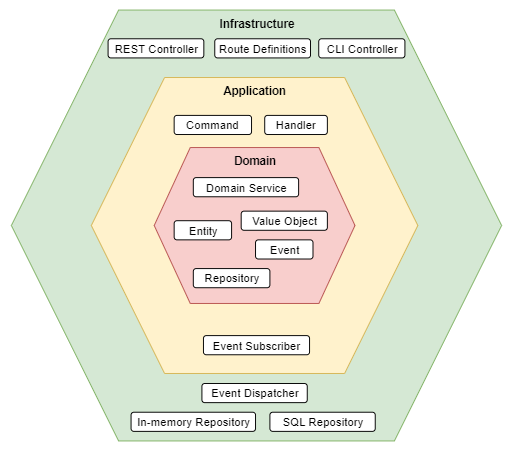
\includegraphics[scale=0.7]{Imagens/chap04/building-blocks-hexagon.png}
  \caption{Building blocks on the Hexagonal Architecture.}
  \label{fig:building-blocks-hexagon}
\end{figure}

\autoref{fig:building-blocks-sequence-diagram} exemplifies the interaction and communication between the defined building blocks. It illustrates the complete execution flow of the \textit{assign task} use case from the Service Work back end. Domain, Application and Infrastructure components are represented in red, yellow and green, respectively.

\begin{figure}[htbp]
  \centering
  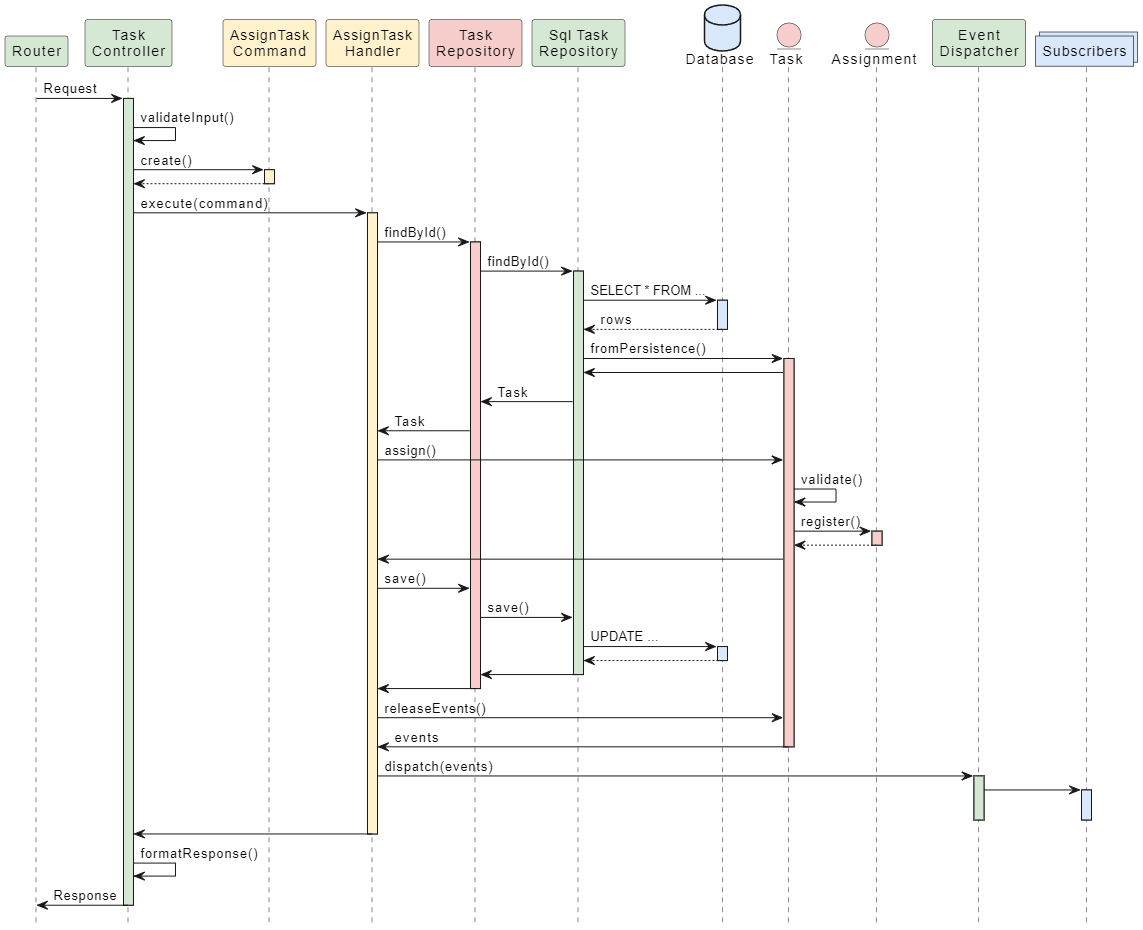
\includegraphics[scale=0.37]{Imagens/chap04/building-blocks-sequence-diagram.png}
  \caption{Sequence diagram of the \textit{assign task} use case.}
  \label{fig:building-blocks-sequence-diagram}
\end{figure}

First, an HTTP request is made to the server, and after passing by all middleware, the \texttt{Router} redirects the request to the proper \texttt{TaskController}. The request body content is validated. Next, the controller creates an \texttt{AssignTaskCommand} object based on the request and uses it to execute the \texttt{AssignTaskHandler}. The command handler calls the \texttt{TaskRepositroy}. In this case, it is implemented by the \texttt{SqlTaskRepository}, which queries through the database to get the specific task that the member is being assigned. Using the raw data, the SQL repository implementation rebuilds the entire \textit{Task} aggregate, including the \texttt{Task} and \texttt{Assignment} entities.

The handler calls the \texttt{assign} method on the aggregate root, which performs all the checks to guarantee all domain constraints, and it creates a new \texttt{Assignment} internally. After successfully assigning the task to a member on the domain layer, the command handler calls the repository again, this time to persist the entire Task aggregate. Next, all the events from the aggregate are released and dispatched through the \texttt{EventDispatcher} to the \texttt{Subscribers} that will, for example, notify the member about the new assignment and recalculate the total assigned FTE for the ALICE collaboration during the current year. Finally, the controller formats a response returned to the router and sent back to the client.
